\documentclass{article}
\usepackage{fullpage}
%%% Работа с русским языком
\usepackage[T2A]{fontenc}
\usepackage[utf8]{inputenc}
\usepackage[english,russian]{babel}   %% загружает пакет многоязыковой вёрстки
\usepackage{indentfirst}
\frenchspacing
\usepackage{titlesec} % package to customize chapters, sections and subsections style
%--------------------------------------
\titleformat{\section}{\large\bfseries\centering}{\thesection}{1em}{}
%Hyphenation rules
%--------------------------------------
\usepackage{hyphenat}
\hyphenation{мате-мати-ка восста-навливать}
%--------------------------------------
\usepackage[intlimits,sumlimits]{amsmath}
\usepackage{amsfonts,amssymb,amsthm,mathtools}
\usepackage[bb=pazo,frak=pxtx,frakscaled=1.3]{mathalfa}
\usepackage{upgreek}
\usepackage{graphicx}
\usepackage{verbatim} %% для многострочных комментариев

%% Перенос знаков в формулах (по Львовскому)
\newcommand*{\hm}[1]{#1\nobreak\discretionary{}
{\hbox{$\mathsurround=0pt #1$}}{}}

\renewcommand{\le}{\ensuremath{\leqslant}}
\renewcommand{\leq}{\ensuremath{\leqslant}}
\renewcommand{\ge}{\ensuremath{\geqslant}}
\renewcommand{\geq}{\ensuremath{\geqslant}}

\title{Контрольная работа №4 по курсу «Математика»\\
Тема: «Кратные интегралы»\\
Вариант №1}
\author{Ригованов Филипп Юрьевич, студент группы КТбз1-1}
\begin{document}
\date{}
\maketitle
\section*{Задание № 1.}
Изменить порядок интегрирования в повторном интеграле. Изобразить область интегрирования.

$$\int\limits_{0}^{1} dy \int\limits_{\sqrt{y}-1}^{1-y} f(x,y)\;dx.$$
\begin{center}Решение:\end{center}
\begin{center}
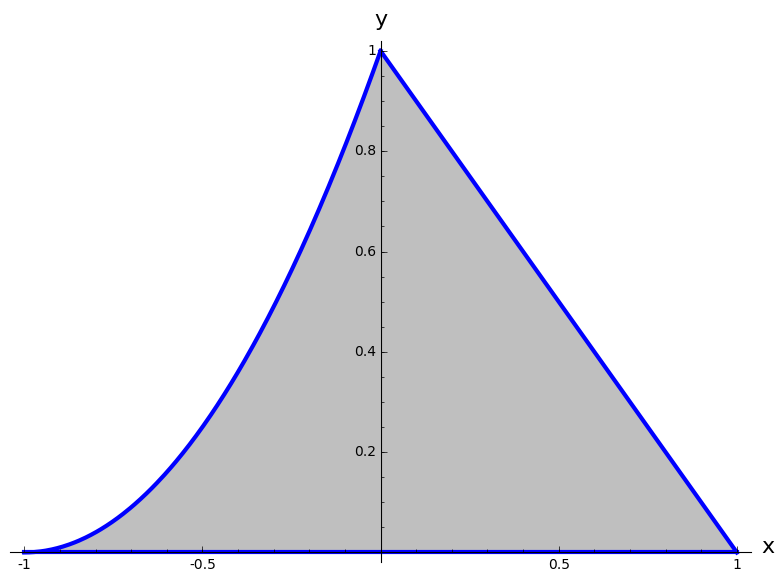
\includegraphics[width=300pt,natwidth=784,natheight=582]{/Users/phil/my/tex/src/math_1.png}
\end{center}
$$\int\limits_{0}^{1} dy \int\limits_{\sqrt{y}-1}^{1-y} f(x,y)\;dx=\int\limits_{-1}^{0} dx \int\limits_{0}^{(x+1)^2} f(x,y)\;dy+\int\limits_{0}^{1} dx \int\limits_{0}^{1-x} f(x,y)\;dy.$$

\section*{Задание № 2.}
Вычислить двойной интеграл $\iint\limits_{D} f(x,y)dx dy$ по области $D$, ограниченной заданными кривыми. $f(x,y)=3x^2y+2x,\quad \partial D:\; y^3=x,\; 4y=x,\; x\geq0$.
\begin{center}Решение:\end{center}

$$\iint\limits_{D} \left(3x^2y+2x\right) dx dy=\frac{1}{2}x^2 y (x y+2)=
\int\limits_{0}^{2} dy \int\limits_{y^3}^{4y} \left(3x^2y+2x\right)\;dx=
\int\limits_{0}^{2} \left(\left(x^3y+x^2\right)\bigg|\limits_{x=y^3}^{4y}\right) dy =$$
$$= \int\limits_{0}^{2} \left( 64y^4+16y^2-y^{10}-y^6\right) dy = \left(\frac{64y^5}{5}+\frac{16y^3}{3}-\frac{y^{11}}{11}-\frac{y^7}{7}\right)\bigg|\limits_{0}^{2} = \frac{2^{11}}{5}+\frac{2^7}{3}-\frac{2^{11}}{11}-\frac{2^7}{7}=$$

$$=\frac{286208}{1155}\approx247.799.$$

\section*{Задание № 3.}
С помощью двойного интеграла найти площадь фигуры, определенной в полярных координатах указанными неравенствами. $\rho\leq 3\sin{2\varphi}$.
\begin{center}Решение:\end{center}
\begin{center}
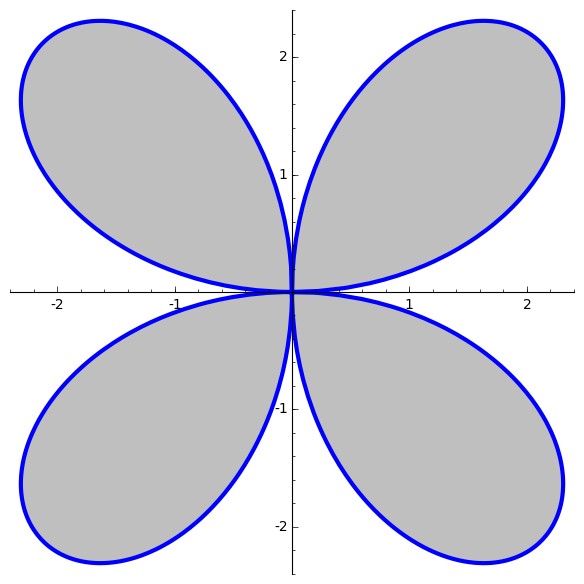
\includegraphics[width=200pt,natwidth=584,natheight=584]{/Users/phil/my/tex/src/math_3.png}
\end{center}
Фигура ограничена четырьмя одинаковыми лепестками, значит её площадь равна умноженной на четыре площади одного лепестка.

$$S=4\iint\limits_{D}\rho \, d\rho d\varphi=4\int\limits_{0}^{\frac{\pi}{2}}d\varphi\int\limits_{0}^{3\sin{2\varphi}}\rho \, d\rho=2\int\limits_{0}^{\frac{\pi}{2}}\rho^2\bigg|\limits_{0}^{3\sin{2\varphi}}d\varphi=18\int\limits_{0}^{\frac{\pi}{2}}(\sin^2{2\varphi}) \; d\varphi=9\int\limits_{0}^{\frac{\pi}{2}}(1-\cos{4\varphi}) \; d\varphi=$$
$$=9\left(\varphi-\frac{1}{4}\sin4\varphi\right)\bigg|\limits_{0}^{\frac{\pi}{2}}=\frac{9\pi}{2}.$$


\section*{Задание № 4.}
 Вычислить тройной интеграл $\iiint\limits_{V} f(x,y,z)dx dy dz$ от заданной функции $f(x,y,z)$ по области $V$, ограниченной указанными поверхностями.
 $f(x,y,z)=2x+y-z,\quad \partial V:\; 2x+y-z-2=0,\;x=0,\;\\y=0,\;z=0$.
 \begin{center}Решение:\end{center}

$$\iiint\limits_{V}(2x+y-z)\;dx dy dz=\int\limits_{0}^{1}dx\int\limits_{0}^{2-2x}dy\int\limits_{2x+y-2}^{0}(2x+y-z)dz=\int\limits_{0}^{1}dx\int\limits_{0}^{2-2x}\left((2x+y)z-\frac{z^2}{2}\right)\bigg|\limits_{z=2x+y-2}^{0}dy=$$
$$=\int\limits_{0}^{1}dx\int\limits_{0}^{2-2x}\left(\frac{(2x+y-2)^2}{2}-(2x+y)(2x+y-2)\right)dy=\int\limits_{0}^{1}dx\int\limits_{0}^{2-2x}\left(2-2x^2-2xy-\frac{y^2}{2}\right)dy=$$
$$=\int\limits_{0}^{1}\left(2y-2x^2y-xy^2-\frac{y^3}{6}\right)\bigg|\limits_{y=0}^{2-2x}dx=\int\limits_{0}^{1}(2-2x)\left(2-2x^2-x(2-2x)-\frac{(2-2x)^2}{6}\right)dx=\int\limits_{0}^{1}\left(\frac{4x^3}{3}-4x+\frac{8}{3}\right)dx=$$
$$=\left(\frac{x^4}{3}-2x^2+\frac{8x}{3}\right)\bigg|\limits_{0}^{1}=\frac{1}{3}-2+\frac{8}{3}=1.$$
P.S. В методичке это задание решено с ошибкой.
\begin{comment}
\section*{Задание № 5.}
Вычислить тройной интеграл $\iiint\limits_{V} f(x,y,z)dx dy dz$, перейдя к сферической системе координат, где $V$ - область, ограниченная указанными поверхностями.
$f(x,y,z)=\frac{1}{z},\quad \partial V:\; x^2+y^2+z^2=1,\;\\x^2+y^2+z^2=4,\;z=1,\;x\geq0,\;y\geq0,\;z\geq0$.
\begin{center}Решение:\end{center}

$$\iiint\limits_{V} \frac{1}{z} dx dy dz=\begin{vmatrix} x=\rho\sin{\theta}\cos{\varphi} \\ y=\rho\sin{\theta}\sin{\varphi} \\ z=\rho\cos{\theta} \\ dx dy dz = \rho^2 \sin{\theta} \; d\rho d\varphi d\theta \end{vmatrix}=\int\limits_{0}^{\frac{\pi}{2}}d\varphi\int\limits_{0}^{0}d\theta\int\limits_{0}^{0}\rho \tg{\theta}\;d\rho=$$

\section*{Задание № 6.}
Даны: векторное поле $\vec{F}=P\vec{i}+Q\vec{j}+R\vec{k}$
и плоскость $Ax+By+Cz=0\; (p)$, которая совместно с координатными плоскостями образует пирамиду $V$. Пусть $\sigma$ – основание пирамиды, принадлежащее плоскости $(p)$.
Найти поток векторного поля $\vec{F}$ через поверхность $\sigma$ в направлении внешней нормали.
$$\vec{F}=3x\vec{i}+z\vec{j},\qquad x+2y+2z-2=0.$$
\begin{center}Решение:\end{center}

\end{comment}
\end{document}
